\section{Experiments} 
\label{sec:experiments_009}

In this section, we provide an extensive evaluation set-up for uncertainty quantification for node classification. It compares \textbf{\GPNacro{}} to 13 baselines on 8 datasets and consists in two task types. First, we evaluate the detection of OOD nodes with features perturbations and Left-Out classes. Second, we evaluate the robustness of accuracy, calibration and uncertainty metrics w.r.t. feature and edge shifts.

\subsection{Setup}

\paragraph{Ablation.} In the experiments, \GPNacro{} uses a MLP as feature encoder, radial normalizing flows \citep{radialflow} for the density estimation and a certainty budget $N$ which scales with respect to the latent dimension \citep{NatPN2021}. We provide an ablation study covering aleatoric uncertainty through APPNP, feature-level estimates through PostNet, diffusing resulting pseudo-counts after training, and \GPNacro{} with diffusion of \smash{$\log(\beta_\iclass^{\text{ft}, (\nodev)})$} instead of \smash{$\beta_\iclass^{\text{ft}, (\nodev)}$} (see \cref{sec:ablation-study_009}). The complete \GPNacro{} model outperforms the ablated models for uncertainty estimation. Further, we provide a hyper-parameter study covering for example different number of flow layers, latent dimensions, PPR teleport probabilities (see \cref{sec:hyperparameter-study})). 

\paragraph{Baselines.} We used 13 baselines covering a wide variety of models for semi-supervised node classification and uncertainty estimation. We show the results of 5 baselines in the main paper and the full results in appendix. It contains two standard GNNs (i.e. Vanilla GCN \textbf{VGCN} \citep{Kipf2016, Shchur2018} and \textbf{APPNP} \citep{Klicpera2018}), one robust GNN (i.e. \textbf{RGCN} \citep{Zhu2019}), one dropout-based method for GNN (i.e. \textbf{DropEdge} \citep{Rong2019}), two Graph Gaussian Processes methods (i.e. \textbf{GGP} \citep{Ng2018} and \textbf{Matern-GGP} \citep{Borovitskiy2020}), the Graph-based Kernel Dirichlet GCN method (i.e. \textbf{GKDE-GCN} \citep{Zhao2020}) and two parameter-less methods (i.e. \textbf{GKDE} \citep{Zhao2020} and Label Propagation \textbf{LP} see \cref{sec:app_model_details}). Further, we also compared to direct adaptation of dropout (i.e. \textbf{VGCN-Dropout}\citep{dropout}), ensemble (i.e. \textbf{VGCN-Ensemble} \citep{ensembles}), BNN (i.e. \textbf{VGCN-BNN} \citep{bayesian-networks}) and energy-based models (i.e. \textbf{VGCN-Energy} \citep{Liu2020a}) to vanilla GCNs. All models are trained using the same number of layers and similar number of hidden dimensions. We used early stopping and report the used hyperparameters in appendix. The results are averaged over 10 initialization seeds per split. Further model details are given in appendix.

\paragraph{Datasets.} We used 8 datasets with different properties summarized in appendix. We show the results of 3 datasets in the main part of this chapter and the full results in appendix. It contains common citation network datasets (i.e. \textbf{CoraML} \citep{Mccallum2000, Giles1998, Getoor2005, Sen2008a}, \textbf{CiteSeer} \citep{Giles1998, Getoor2005, Sen2008a}, \textbf{PubMed} \citep{Namata2012}, \textbf{CoauthorPhysics} \citep{Shchur2018} \textbf{CoauthorCS} \citep{Shchur2018})
 and co-purchase datasets (i.e. \textbf{AmazonPhotos} \citep{Mcauley2015, Shchur2018}, \textbf{AmazonComputers} \citep{Mcauley2015, Shchur2018}). The results are averaged over 10 initialization splits with a train/val/test split of $5\%/15\%/80\%$ using stratified sampling. Further, we evaluate on the large \textbf{OGBN Arxiv} dataset with $169,343$ nodes and $2,315,598$ edges \citep{ogb-dataset, microsoft-academic-graph}. Further dataset details are given in the appendix.
 
\subsection{Results}
 
\looseness=-1
\paragraph{OOD Detection.} In this section, we evaluate uncertainty estimation for OOD detection. To this end, we use the Area Under Receiving Operator Characteristics Curve (AUC-ROC) with aleatoric scores \smash{$u_\text{alea}\nodeidxv$} \textbf{(Alea)} and epistemic scores \smash{$u_\text{epist}\nodeidxv$} \textbf{(Epist)} similarly to \citep{charpentier2020, Zhao2020, PriorNetworks, reverse-kl, distribution-distillation, Liu2020a}. For \GPNacro{}, we differentiate between epistemic uncertainty scores without network effects \textbf{(w/o Net.)} and with network effects \textbf{(w/ Net.)}. Further, we report results with the Area Under the Precision-Recall Curve (AUC-PR) in appendix. The definition of OOD for nodes in the presence of feature and network information is more complex than for i.i.d. input features. Hence, we propose two types of OOD nodes: nodes with OOD feature perturbations and nodes from Left-Out classes. For feature perturbations, we compute the accuracy on the perturbed nodes \textbf{(OOD-Acc)} to evaluate if the model can correct anomalous features. For Left-Out classes, we compute the accuracy on the observed classes \textbf{(ID-Acc)}. We report the short results in \cref{tab:ood_short}. We set a threshold of 64 GiB and 12 hours per training run. We also exclude methods which do not use attributes for detection of OOD feature perturbations. 


\textit{\underline{Feature perturbations:}} These perturbations aim at isolating the contribution of the node feature information on the model predictions. To this end, we randomly select a subset of the nodes. For each single node $\nodev$, we perturb individually its features using a Bernoulli or a Normal distribution (i.e. $\x\nodeidxv \sim \DBer(0.5)$ and $\x\nodeidxv \sim \DNormal(\veczero, \vecone)$) keeping all other node features fixed. We then compare the uncertainty prediction on the perturbed and unperturbed node. On one hand, Bernoulli noise corresponds to small perturbations in the domain of discrete bag-of-words features. On the other hand, Normal noise corresponds to extreme perturbations out of the domain of discrete bag-of-words features. In practice, we expect out-of-domain perturbations to be easily detected \citep{charpentier2020}. First, we remark that uncertainty estimates of \GPNacro{} based on features achieves an absolute improvement of at least $+15\%$ and $+29\%$ for Bernoulli and Normal perturbations over all baselines using network effects. This shows that \GPNacro{} disentangles well the uncertainty without and with network effects. Second, we remark that all uncertainty estimates with network effects achieve poor results. This is expected if models can recover the correct prediction after aggregation steps. Specifically, we observe that \GPNacro{} achieves an accuracy improvement between $+16\%$ and $+64\%$ for Normal perturbations on perturbed nodes compared to baselines. It stresses that \GPNacro{} performs a consistent evidence aggregation from neighborhood to recover from anomalous features. Further, note that \GPNacro{} is still capable to detect those perturbed nodes almost perfectly using feature uncertainty. These remarks aligns with des.~\ref{ax:certainty_features}. 


\textit{\underline{Left-Out classes:}} Detection of Left-Out classes involves both feature and neighborhood information. In this case, we remove the Left-Out classes from the training set but keep them in the graph similarly to \citep{Zhao2020}. We observe that the uncertainty estimates with network effects of \GPNacro{} achieves an absolute improvement between $+12\%$ and $+16\%$ compared to its uncertainty estimates without network effects. It highlights the benefit of incorporating network information for uncertainty predictions when OOD samples (i.e. samples from the Left-Out classes) are likely to be connected to each other. This remark aligns with des.~\ref{ax:certainty_network_epistemic}. Further, \GPNacro{} outperforms other baselines by $+2\%$ to $+22\%$ for LOC detection while maintaining a competitive accuracy on other classes.

\textit{\underline{Misclassified samples:}} In addition to the OOD scores, we also report the results for the detection of misclassified samples with aleatoric and epistemic uncertainty on several datasets and models in \cref{sec:add-exp-misclassification} for the sake of completeness. GPN performs competitively with the baselines. Moreover, we observe that epistemic uncertainty is better for OOD detection and aleatoric uncertainty is better for misclassification detection as already observed  e.g. in \citep{Zhao2020}.

%Note that related work like \citep{Zhao2020, Malinin2018, Charpentier2020} evaluates the quality of aleatoric uncertainty estimates through misclassification experiments which allows for a broader range of uncertainty measures. As we focus on measures directly derived from the categorical distribution, we evaluate aleatoric uncertainty indirectly through measures of calibration. Furthermore with a focus on epistemic uncertainty, we cover corresponding measures and experiments exhaustively with aleatoric uncertainty only given for reference to allow a comparison to models without any intrinsic measures of epistemic uncertainty. To facilitate a fair comparison with related work, we also present results for misclassification experiments in the appendix.

\begin{table*}[!h]
    \centering
    %\tiny
    \resizebox{\textwidth}{!}{
    \begin{tabular}{ll|cl|cl|cl}
        \toprule
        & \textbf{Model} & \textbf{ID-ACC} & \textbf{OOD-AUC-ROC} & \textbf{OOD-ACC} & \textbf{OOD-AUC-ROC} & \textbf{OOD-ACC} & \textbf{OOD-AUC-ROC} \\
        & & \multicolumn{2}{c|}{Leave-Out Classes} & \multicolumn{2}{c|}{{$\x\nodeidxv \sim \DBer(0.5)$}} & \multicolumn{2}{c}{$\x\nodeidxv \sim \DNormal(0,1)$} \\
        \midrule
        
        %\hphantom{0}
        %$\hphantom{00.00}$

        \multirow{6}{*}{CoraML} 
        & Matern-GGP & ${87.03}$ & ${83.13}$  /  ${82.98}$  /  $n.a.$ & $n.a.$ & $\hphantom{00.00}$ $n.a.$ $\hphantom{00.00}$ & $n.a.$ & $\hphantom{00.00}$ $n.a.$ $\hphantom{00.00}$ \\
        & VGCN-Dropout & ${89.08}$ & ${81.27}$ / ${71.65}$ / $n.a.$ & ${77.76}$ & ${62.06}$ / ${50.38}$ / $n.a.$ & ${18.28}$ & ${40.53}$ / ${{71.06}}$ / $n.a.$\\
        & VGCN-Energy & ${89.66}$ & ${81.70}$ / ${83.15}$ / $n.a.$ & ${78.90}$ & ${{63.68}}$ / ${{66.26}}$ / $n.a.$ & ${18.37}$ & ${\hphantom{0}9.34}$ / ${\hphantom{0}0.32}$ / $n.a.$\\
        & VGCN-Ensemble & ${\mathbf{89.87}}$ & ${81.85}$ / ${74.24}$ / $n.a.$ & ${78.00}$ & ${63.58}$ / ${56.81}$ / $n.a.$ & ${21.00}$ & ${33.72}$ / ${64.92}$ / $n.a.$\\
        & GKDE-GCN & ${89.33}$ & ${82.23}$ / ${82.09}$ / $n.a.$ & ${76.40}$ & ${61.74}$ / ${63.15}$ / $n.a.$ & ${16.86}$ & ${40.03}$ / ${\hphantom{0}1.42}$ / $n.a.$\\
        & GPN & ${88.51}$ & ${{83.25}}$ / ${\mathbf{86.28}}$ / ${{80.95}}$ & ${\mathbf{80.98}}$ & ${57.99}$ / ${55.23}$ / ${\mathbf{89.47}}$ & ${\mathbf{81.53}}$ & ${55.96}$ / ${56.51}$ / ${\mathbf{100.00}}$\\

        \midrule

        \multirow{6}{*}{\shortstack{Amazon \\ Photos}}
        & Matern-GGP & ${88.65}$ & ${{87.26}}$ / ${86.75}$ / $n.a.$ & $n.a.$ & $\hphantom{00.00}$ $n.a.$ $\hphantom{00.00}$ & $n.a.$ & $\hphantom{00.00}$ $n.a.$ $\hphantom{00.00}$\\
        & VGCN-Dropout & ${94.04}$ & ${80.90}$ / ${70.11}$ / $n.a.$ & ${83.86}$ & ${56.85}$ / ${55.04}$ / $n.a.$ & ${22.29}$ & ${49.11}$ / ${66.74}$ / $n.a.$\\
        & VGCN-Energy & ${94.24}$ & ${82.44}$ / ${79.64}$ / $n.a.$ & ${83.91}$ & ${57.91}$ / ${59.07}$ / $n.a.$ & ${21.40}$ & ${31.07}$ / ${\hphantom{0}6.42}$ / $n.a.$\\
        & VGCN-Ensemble & ${\mathbf{94.28}}$ & ${82.72}$ / ${88.53}$ / $n.a.$ & ${84.40}$ & ${57.86}$ / ${56.01}$ / $n.a.$ & ${20.30}$ & ${44.14}$ / ${69.01}$ / $n.a.$\\
        & GKDE-GCN & ${89.84}$ & ${73.65}$ / ${69.09}$ / $n.a.$ & ${73.17}$ & ${57.01}$ / ${58.00}$ / $n.a.$ & ${24.04}$ & ${24.45}$ / ${\hphantom{0}9.82}$ / $n.a.$\\
        & GPN & ${94.01}$ & ${82.72}$ / ${\mathbf{91.98}}$ / ${76.57}$ & ${\mathbf{87.47}}$ & ${56.25}$ / ${60.52}$ / $\mathbf{75.24}$ & ${\mathbf{88.29}}$ & ${51.89}$ / ${61.89}$ / $\mathbf{100.00}$\\
        
        \midrule
        
        \multirow{6}{*}{\shortstack{OGBN \\ Arxiv}}
        & Matern-GGP & $n.f.$ & $\hphantom{00.00}$ $n.f.$ $\hphantom{00.00}$ & $n.f.$ &$ \hphantom{00.00}$ $n.f.$ $\hphantom{00.00}$ & $n.f.$ & $\hphantom{00.00}$ $n.f.$ $\hphantom{00.00}$\\
        & VGCN-Dropout & ${75.47}$ & ${65.35}$ / ${64.24}$ / $n.a.$ & ${65.30}$ & ${48.11}$ / ${50.64}$ / $n.a.$ & ${49.90}$ & ${{60.10}}$ / ${62.87}$ / $n.a.$\\
        & VGCN-Energy & ${75.61}$ & ${64.91}$ / ${64.50}$ / $n.a.$ & ${65.70}$ & ${46.16}$ / ${48.54}$ / $n.a.$ & ${{51.30}}$ & ${53.83}$ / ${48.53}$ / $n.a.$\\
        & VGCN-Ensemble & ${\mathbf{76.12}}$ & ${65.93}$ / ${70.77}$ / $n.a.$ & ${\mathbf{67.00}}$ & ${45.99}$ / ${47.41}$ / $n.a.$ & ${49.00}$ & ${59.94}$ / ${{66.44}}$ / $n.a.$\\
        & GKDE-GCN & ${73.89}$ & ${{68.84}}$ / ${72.44}$ / $n.a.$ & ${65.20}$ & ${{50.98}}$ / ${{51.31}}$ / $n.a.$ & ${45.40}$ & ${53.94}$ / ${55.28}$ / $n.a.$\\
        & GPN & ${73.84}$ & ${66.33}$ / ${\mathbf{74.82}}$ / ${{62.17}}$ & ${65.50}$ & ${{51.49}}$ / ${{55.82}}$ / ${\mathbf{93.05}}$ & ${\mathbf{65.50}}$ & ${51.43}$ / ${55.85}$ / ${\mathbf{95.54}}$\\
        \bottomrule
    \end{tabular}
    }
    \caption{LOC and Feature Perturbations: Accuracy is reported on ID nodes for LOC experiments and on OOD nodes for feature perturbation experiments. OOD-AUC-ROC scores are given as \emph{[Alea w/ Net] / [Epist w/ Net] / [Epist w/o Net]}. $n.a.$ means either model or metric not applicable and $n.f.$ means not finished within our constraints.}
    \label{tab:ood_short}
    \vspace{-3mm}
\end{table*}

\looseness=-1
\paragraph{Attributed Graph Shifts.} In this section, we focus on evaluating the robustness of the accuracy, calibration and the evolution of the uncertainty estimation under node feature shifts and edges shifts. This aligns with \citep{dataset-shift} which aims at evaluating the reliability of uncertainty estimates under dataset shifts for i.i.d. inputs. Specifically, we evaluates the evolution of the accuracy, the ECE \citep{Naeini2015} calibration score, the epistemic and the aleatoric uncertainty measures. 


\textit{\underline{Feature shifts:}} We perturbed the features of a fraction of the nodes using unit Gaussian perturbations. We report the short results in \cref{fig:shifts-normal-cora} and the full results in appendix. On one hand, we observe that \GPNacro{} is significantly more robust to feature perturbations than all baselines. Indeed, the accuracy of \GPNacro{} decreases by less than $5\%$ even when $80\%$ of the nodes are perturbed while the accuracy of other baselines decreases by more than $50\%$ when only $20\%$ of the nodes are perturbed. Similarly, we observed that \GPNacro{} remains calibrated even when a high fraction of nodes are perturbed contrary to baselines. Hence, \GPNacro{} intuitively discards uncertain features from perturbed nodes and only accounts for certain features from other nodes for more accurate predictions. On the other hand, we observe that, as desired, the average epistemic uncertainty of \GPNacro{} consistently decreases when more nodes are perturbed. This remark aligns with des.~\ref{ax:certainty_network_epistemic}. In contrast, baselines dangerously become more certain while achieving a poorer accuracy similarly to ReLU networks \citep{overconfident-relu}. Hence \GPNacro{} predictions are significantly more reliable than baselines under feature shifts. 


\textit{\underline{Edge shifts:}} For edge shifts, we perturbed a fraction of edges at random. We report the results in appendix. As desired, we observe that the aleatoric uncertainty increases for all models including \GPNacro{}. This aligns with des.~\ref{des:certainty_network_aleatoric} and the expectations that conflicting neighborhood should lead to more aleatorically uncertain predictions. Furthermore, the average epistemic uncertainty of \GPNacro{} remains constant which is reasonable since the average evidence of a node's neighborhood remains constant.

%
\begin{figure}[!h]
    \centering
    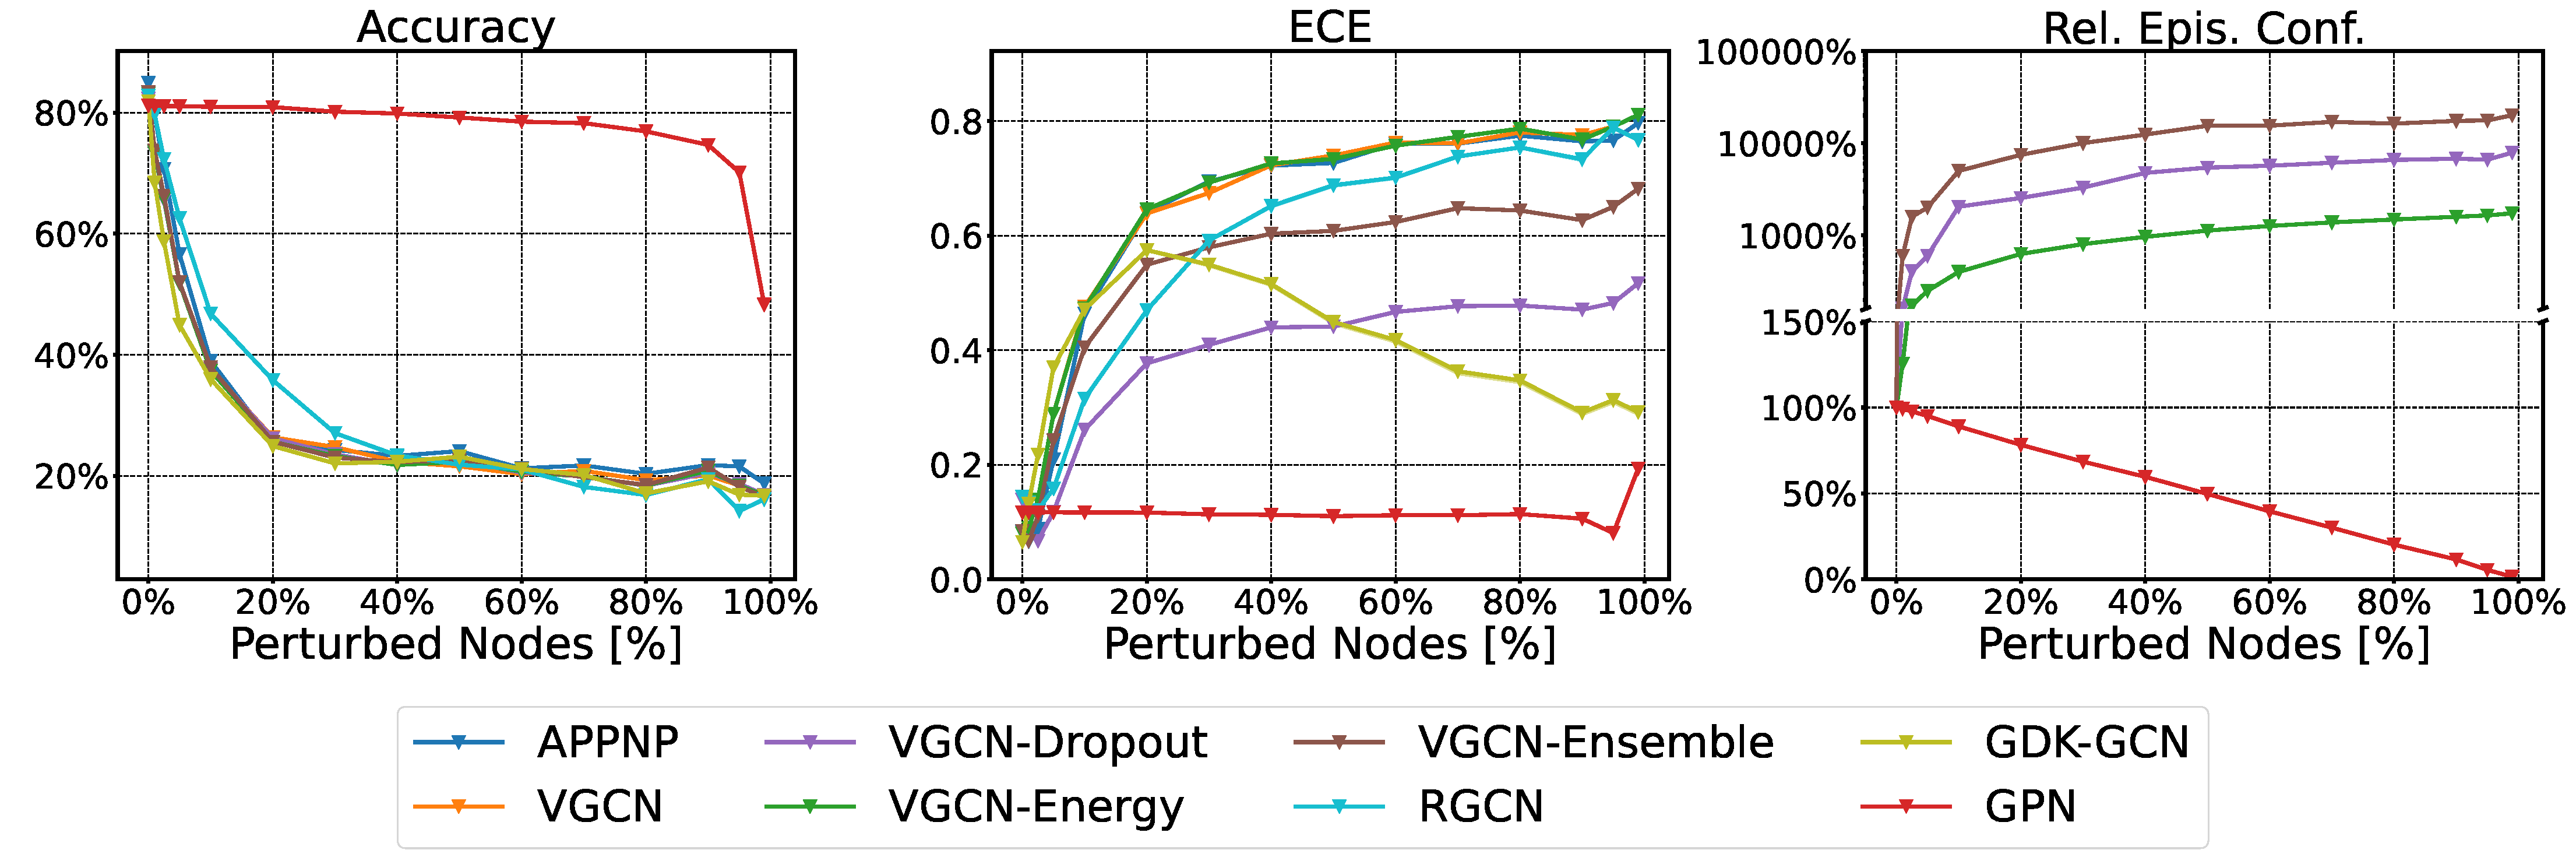
\includegraphics[width=\textwidth]{sections/009_neurips2021/resources/CoraML-normal-shift.pdf}
    \caption{Accuracy, ECE, and average epistemic confidence under feature shifts for CoraML. We perturb features of different percentage of nodes using a Unit Gaussian noise.}
    \label{fig:shifts-normal-cora}
\end{figure}
%

\paragraph{Qualitative Evaluation.} We show the abstracts of the CoraML papers achieving the highest and the lowest epistemic uncertainty without network effects in \cref{tab:odd_abstracts} and in the appendix. Interestingly, we observed that most uncertain papers corresponds to short and unconventional abstracts which can be seen as anomalous features. Furthermore, we also ranked the nodes w.r.t. to their epistemic uncertainty with network effects. In this case, we observed that $78/100$ nodes with the highest uncertainty do not belong to the largest connected component of the CoraML dataset. We propose additional uncertainty visualizations for \GPNacro{} in \cref{sec:add-exp-qualitative}. 

\paragraph{Inference \& training time.} We provide a comparison of inference and training times for most of the datasets and models under consideration in \cref{sec:add-exp-time}. GPN needs a single pass for uncertainty estimation but requires the additional evaluation of one normalizing flow per class compared to APPNP. Hence, GPN brings a small computational overhead for uncertainty estimation at inference time. Furthermore, GPN is usually converging relatively fast during training and does not require pre-computing kernel values. In contrast, GKDE-GCN \citep{Zhao2020} requires the computation of the underlying Graph Kernel with a complexity of $\mathcal{O}\left(\nnodes^2\right)$ where $\nnodes$ is the number of nodes in the graph. Finally, GPN is significantly more efficient than dropout or ensemble approaches as it does not require training or evaluating multiple models.

\begin{table}[!h]
    \centering
    \tiny
    \begin{tabular}{p{6.5cm} p{6.5cm}}
        \toprule
        {\tt IlliGAL Report No. 95006 July 1995} & 
        {\tt Report of the 1996 Workshop on Reinforcement} \\
        \midrule
        {\tt Reihe FABEL-Report Status: extern Dokumentbezeichner: Org/Reports/nr-35 Erstellt am: 21.06.94 Korrigiert am: 28.05.95 ISSN 0942-413X} & 
        {\tt We tend to think of what we really know as what we can talk about, and disparage knowledge that we can't verbalize. [Dowling 1989, p. 252]} \\
        \midrule
        {\tt Keith Mathias and Darrell Whitley Technical Report CS-94-101 January 7, 1994} & 
        {\tt Multigrid Q-Learning Charles W. Anderson and Stewart G. Crawford-Hines Technical Report CS-94-121 October 11, 1994} \\
        \midrule
        {\tt Internal Report 97-01} & {\tt A Learning Result for Abstract} \\
        \bottomrule
        \vspace{0.1cm}
    \end{tabular}
    \caption{A selection of abstracts from CoraML which are assigned low feature evidences by GPN.}
    \label{tab:odd_abstracts}
    \vspace{-3mm}
\end{table}
